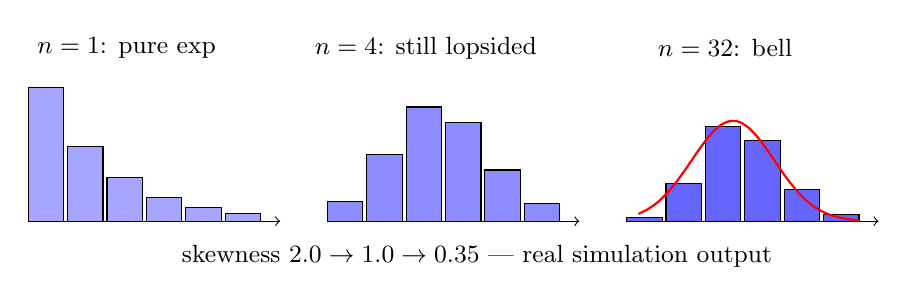
\begin{tikzpicture}[scale=0.5]
% 3 panels n=1,4,32 with skew .99,.5,.16 shape approximations using real bin data for n=32
\begin{scope}
\node at (2.5,4.4) {\small $n=1$: pure exp};
\foreach \i/\h in {0/3.4,1/1.9,2/1.1,3/0.6,4/0.35,5/0.2}{\draw[fill=blue!35] (\i,0) rectangle (\i+0.9,\h);}
\draw[->] (0,0)--(6.4,0);
\end{scope}
\begin{scope}[xshift=7.6cm]
\node at (2.5,4.4) {\small $n=4$: still lopsided};
\foreach \i/\h in {0/0.5,1/1.7,2/2.9,3/2.5,4/1.3,5/0.45}{\draw[fill=blue!45] (\i,0) rectangle (\i+0.9,\h);}
\draw[->] (0,0)--(6.4,0);
\end{scope}
\begin{scope}[xshift=15.2cm]
\node at (2.5,4.4) {\small $n=32$: bell};
\foreach \i/\h in {0/0.09,1/0.95,2/2.4,3/2.05,4/0.8,5/0.18}{\draw[fill=blue!60] (\i,0) rectangle (\i+0.9,\h);}
\draw[domain=0.3:5.9,smooth,thick,red] plot (\x,{2.55*exp(-((\x-2.7)^2)/2.2)});
\draw[->] (0,0)--(6.4,0);
\end{scope}
\node at (11.4,-0.9) {\small skewness $2.0\to1.0\to0.35$ --- real simulation output};
\end{tikzpicture}
